\documentclass[aspectratio=169%可调屏宽比16:9(169),4:3(43)
,serif,mathserif]{beamer}
\mode<presentation>{
%\usetheme{default}
%\usetheme{AnnArbor}
%\usetheme{Antibes}
%\usetheme{Bergen}
%\usetheme{Berkeley}
%\usetheme{Berlin}
%\usetheme{Boadilla}
%\usetheme{CambridgeUS}
%\usetheme{Copenhagen}
%\usetheme{Darmstadt}
%\usetheme{Dresden}
%\usetheme{Frankfurt}
%\usetheme{Goettingen}
%\usetheme{Hannover}
%\usetheme{Ilmenau}
%\usetheme{JuanLesPins}
%\usetheme{Luebeck}
\usetheme{Madrid}
%\usetheme{Malmoe}
%\usetheme{Marburg}
%\usetheme{Montpellier}
%\usetheme{PaloAlto}
%\usetheme{Pittsburgh}
%\usetheme{Rochester}
%\usetheme{Singapore}
%\usetheme{Szeged}
%\usetheme{Warsaw}
% As well as themes, the Beamer class has a number of color themes
% for any slide theme. Uncomment each of these in turn to see how it
% changes the colors of your current slide theme.
%\usecolortheme{albatross}
%\usecolortheme{beaver}
%\usecolortheme{beetle}
%\usecolortheme{crane}
%\usecolortheme{dolphin}
%\usecolortheme{dove}
%\usecolortheme{fly}
%\usecolortheme{lily}
%\usecolortheme{orchid}
%\usecolortheme{rose}
%\usecolortheme{seagull}
%\usecolortheme{seahorse}
%\usecolortheme{whale}
%\usecolortheme{wolverine}
%\setbeamertemplate{footline} % To remove the footer line in all slides uncomment this line
%\setbeamertemplate{footline}[page number] % To replace the footer line in all slides with a simple slide count uncomment this line
%\setbeamertemplate{navigation symbols}{} % To remove the navigation symbols from the bottom of all slides uncomment this line
}
\usepackage{adjustbox}
\usepackage{indentfirst} 
\usepackage{amsmath, amsfonts, epsfig, xspace}
\usepackage{algorithm,algorithmic}
\usepackage{beamerthemesplit}
\usepackage{booktabs}
\usepackage{bm}
\usepackage{braket}
\usepackage{calligra}
\usepackage[T1]{fontenc}
\usepackage{fontspec}
\usepackage{ctex}
\usepackage{latexsym}
\usepackage{multicol}
\usepackage{multimedia}
\usepackage{calligra} \DeclareMathAlphabet{\mathcalligra}{T1}{calligra}{m}{n} \DeclareFontShape{T1}{calligra}{m}{n}{<->s*[2.2]callig15}{}
\usepackage{pstricks,pst-node}
\usepackage{ragged2e}
\usepackage{setspace}
\usepackage[normal,tight,center]{subfigure}
\setlength{\subfigcapskip}{-.5em}
\setlength{\parindent}{2em}
\begin{document}
\title{Efficient Exact Verification of Binarized Neural Networks} % The short title appears at the bottom of every slide, the full title is only on the title page
%\author[Chi~Zhiming]{迟智名} % Your name
\institute[LZU] % Your institution as it will appear on the bottom of every slide, may be shorthand to save space
{	
	%Lanzhou University \\ % Your institution for the title page
	%\medskip
	%\textit{chizhm16@lzu.edu.cn} % Your email address
}
	\CTEXoptions[today=old]
	\date{\today} % Date, can be changed to a custom date
\begin{frame}[plain]\vspace{1.5em}
\titlepage\vspace{-0.5cm}
%\centerline{\includegraphics[height=0.30\textheight]{logo.png}}
%\hfill 指导教师:焦桂梅
\end{frame}
\begin{frame}{目录}
\tableofcontents
\end{frame}
\AtBeginSection[]
{
\begin{frame}{\tiny}
\frametitle{目录}
\tableofcontents[currentsection]
\end{frame}
}
%----------------------------------------------------------------------------------------
%	PRESENTATION SLIDES
%----------------------------------------------------------------------------------------

%------------------------------------------------
\section{Introduction} % Sections can be created in order to organize your presentation into discrete blocks, all sections and subsections are automatically printed in the table of contents as an overview of the talk
%------------------------------------------------
\begin{frame}
	\frametitle{Exact Real-valued NN Verification Challenges}
	\begin{itemize}
		\item Unscalability
		\begin{itemize}		
			\item CPU inference: 2ms
			\item Verification (Xiao et al., 2019): 420s  
		\end{itemize}
		\item Unverifiability
		\begin{itemize}
			\item Floating point error makes real-valued NNs unverifiable
			\item Adversarial inputs exist for verified NNs in practice \\
			Kai Jia and Martin Rinard. "Exploiting Verified Neural Networks via Floating Point Numerical Error." arXiv preprint arXiv:2003.03021 (2020).
		\end{itemize}
	\end{itemize}

\end{frame}

\begin{frame}
	\frametitle{Binarized Neural Networks (BNNs)}
	\begin{itemize}
		\item Weights \& activations constrained to be binary
		\item Computational benefits:
		\begin{itemize}
			\item Efficient inference:
			\begin{itemize}
				\item BNN: 600 GOPS/W on FPGA
				\item Floating point: 50 GFLOPS/W on GPU
			\end{itemize}
			\item 32x reduction of memory footprint
			\item Comparable classification accuracy as fp32 networks
		\end{itemize}
		
	\end{itemize}
	
\end{frame}

\begin{frame}
	\frametitle{BNN Verification}
	\begin{itemize}
		\item Binary values support
		\begin{itemize}
			\item exact logical reasoning without floating point error
			\item  $\implies$ exact verification with correctness guarantees
		\end{itemize}
		\item Previous state of the art BNN verifiers are unsatisfactory
		\begin{itemize}
			\item Less scalable than real-valued verifiers: do not scale to CNNs on CIFAR10
			\item No reported evaluation of verifiable robustness
		\end{itemize}
		
	\end{itemize}	

\end{frame}

\section{Efficient Exact Verification of Binarized Neural Networks}
\begin{frame}
	\frametitle{Efficient SAT solving for BNN verification}
	BNN structure
	\begin{figure}
		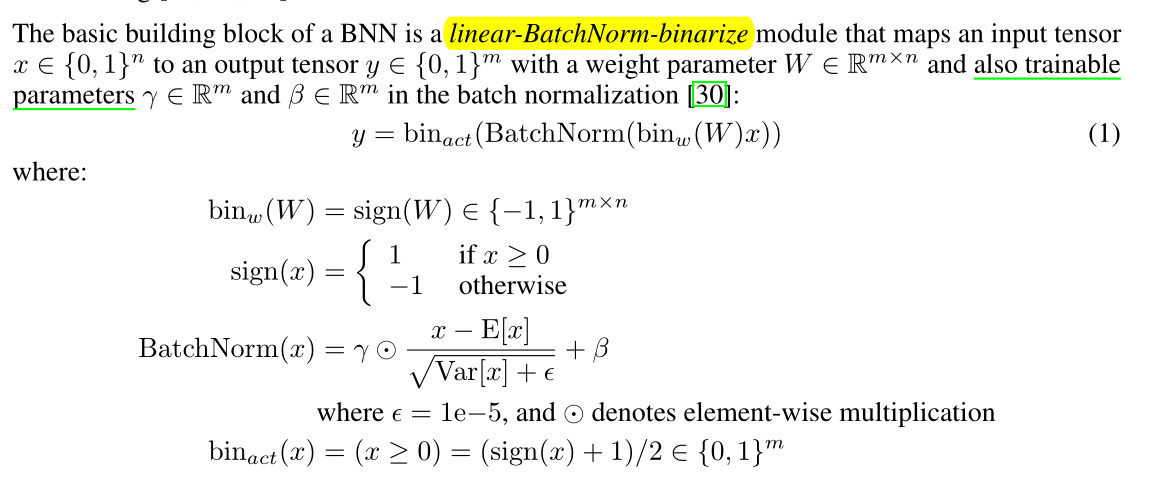
\includegraphics[width=0.7\linewidth]{1.png}
	\end{figure}
	\begin{itemize}
		\item First layer: $x^{\mathrm{q}}=\left\lfloor\frac{x}{s}\right\rceil \cdot s$
		\item Last layer: remove the $bin_{act}$;no softmax;all channel use one mean and var		
	\end{itemize}
\end{frame}

\begin{frame}
	\frametitle{Efficient SAT solving for BNN verification}
	Encoding and Reified cardinality constraints arising in BNN encoding
	For
	$$
	y=\operatorname{bin}_{a c t}\left(k^{\mathrm{BN}} \odot\left(W^{\mathrm{bin}} x\right)+b^{\mathrm{BN}}\right)
	$$
	
	encoding as
	$$
	y_{i}=\left(\sum_{j=1}^{n} l_{i j}\left(x_{j}\right) \gtrless\left[b_{i}\left(k^{\mathrm{BN}}, W^{\mathrm{bin}}, b^{\mathrm{BN}}\right)\right]\right)
	$$

	the untargeted attack goal : $\vee_{i \neq c}\left(y_{i}-y_{c}>0\right)$ \\
	First layer: For $v=\left\lfloor\frac{x}{s}\right\rceil \in \mathbb{Z} \cap[a, b],v=a+\sum_{i=1}^{b-a} t_{i},t_{i} \vee \neg t_{j} \text { for } 1 \leq i<j \leq b-a .$

\end{frame}

\begin{frame}
	\frametitle{Efficient SAT solving for BNN verification}
	\begin{itemize}
		\item Prior work:Encoding as CNF to be solved by an off-the shelf solver
		\item This work:natively solve such constraints by modifying a SAT solver
		\item Result:~100x - ~10,000x speedup compared to the unmodified solver
	\end{itemize}

\end{frame}

\begin{frame}
	\frametitle{Efficient SAT solving for BNN verification}
	Extend a CDCL-based SAT from $\operatorname{MiniSat 2.2}  to \operatorname{MiniSatCS}$.
	\begin{itemize}
		\item CDCL framework: can handle clauses not in the disjunctive form, as long as each clause permits inferring values of undecided variables.
		\item For $y=\left(\sum_{i=1}^{n} l_{i} \leq b\right)$
		\begin{figure}
			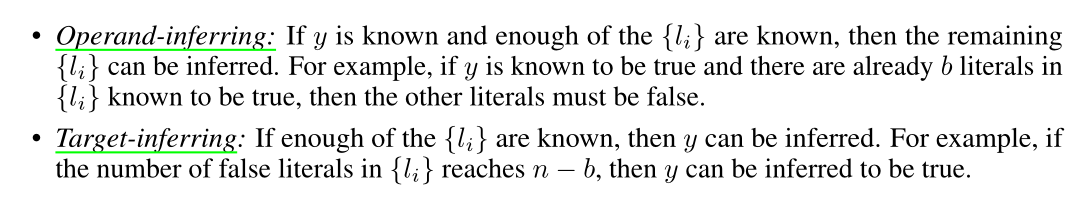
\includegraphics[width=0.8\linewidth]{2.png}
		\end{figure}
	\end{itemize}	
\end{frame}

\begin{frame}
	\frametitle{Efficient SAT solving for BNN verification}
	\begin{figure}
		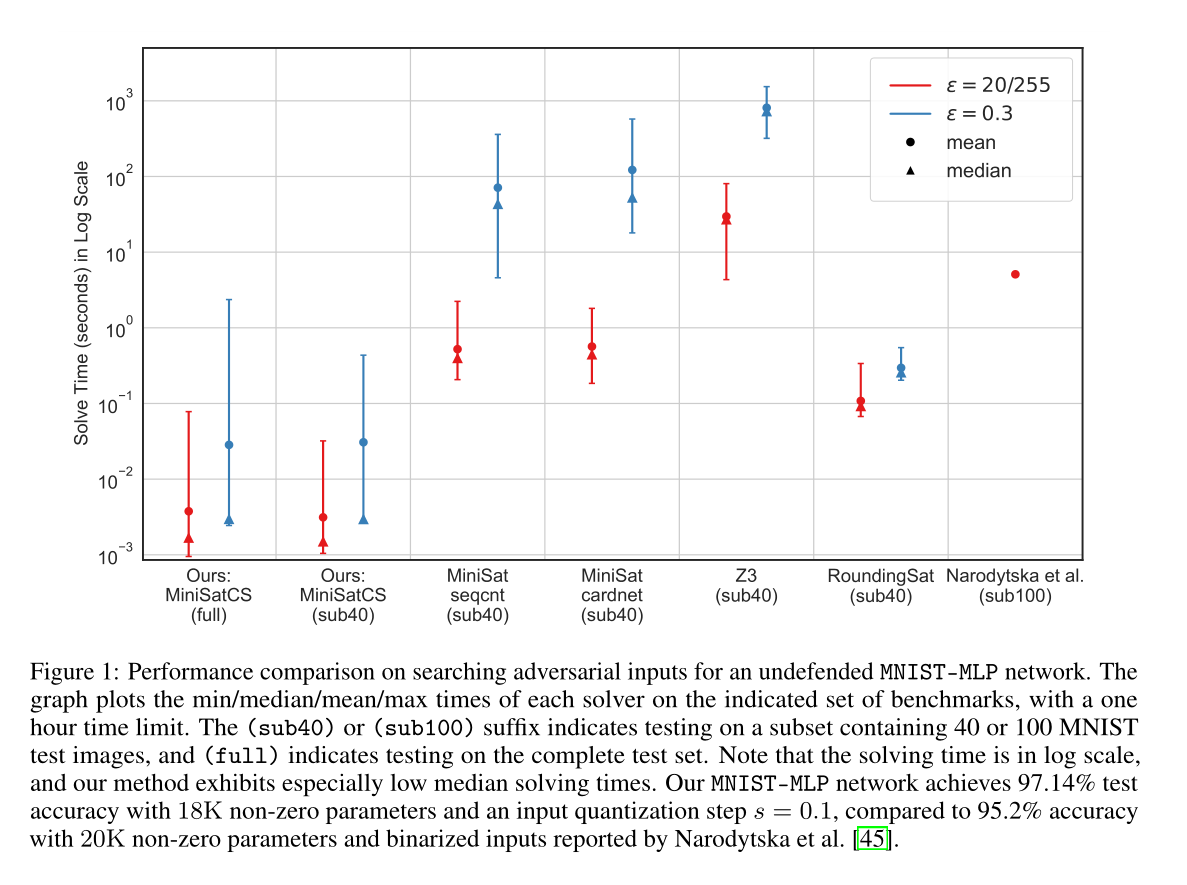
\includegraphics[width=0.68\linewidth]{3.png}
	\end{figure}
	

\end{frame}

\section{Training solver-friendly BNNs}
\begin{frame}
	\frametitle{Balanced layer-wise sparsity}
		\begin{itemize}
			\item Prior work: ternary weights, sparsity concentrates in FC layers
			\item This work: reparameterization with sparse(W) = bin(W) * bin(M) 
			$$
				bin_w(W) = sign(W) \circ \frac{sign(M_w) + 1}{2}
			$$
			\item Result:~100x - ~100,000x verification speedup
\end{itemize}
\end{frame}

\begin{frame}
	\frametitle{Balanced layer-wise sparsity}
	\begin{figure}
		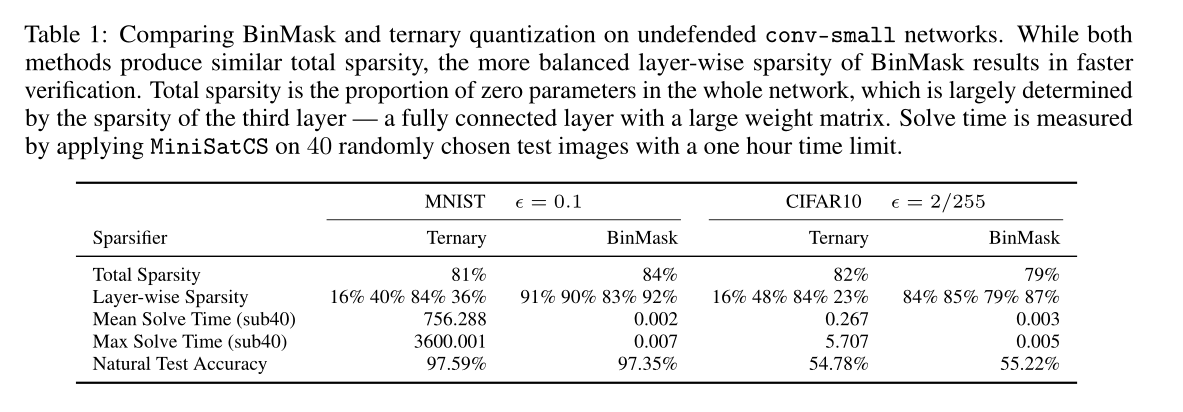
\includegraphics[width=0.9\linewidth]{4.png}
	\end{figure}
\end{frame}
 
\begin{frame}
	\frametitle{Low cardinality bounds}
	\begin{itemize}
		\item A regularizer to induce lower bounds in the cardinality constraints
		\item For $y=\left(\sum_{i=1}^{n} l_{i} \leq b\right)$:
			\begin{itemize}
				\item Converts the constraint into CNF needs $O(nb)$ auxiliary variables and clauses. Thus smallerbproduces a simpler encoding.
				\item $\operatorname{MiniSatCS}$ can infer $y$ to be false once the number of true literals in $\{l_i\}$exceeds $b$, and a smallerbincreases the likelihood of this inference.
				\item If the literals $\left\{l_{i}\right\}$ are drawn from independent symmetrical Bernoulli distributions, then the entropy of $y$ is a symmetrical concave function with respect to $b$ which is maximized when $b=\frac{n}{2}$. Therefore the further $b$ deviates from $\frac{n}{2}$, the more predictable $y$ becomes.
			\end{itemize}
		\item by adding an $L_1$ penalty on the bias terms in cardinality constraints that exceed a threshold $\tau$:
			\begin{equation*}
				L^{\mathrm{CBD}}=\eta \max \left(b\left(k^{\mathrm{BN}}, W^{\mathrm{bin}}, b^{\mathrm{BN}}\right)-\tau, 0\right)
			\end{equation*}			
			
	\end{itemize}
\end{frame}

\begin{frame}
	\frametitle{Low cardinality bounds}
	\begin{figure}
		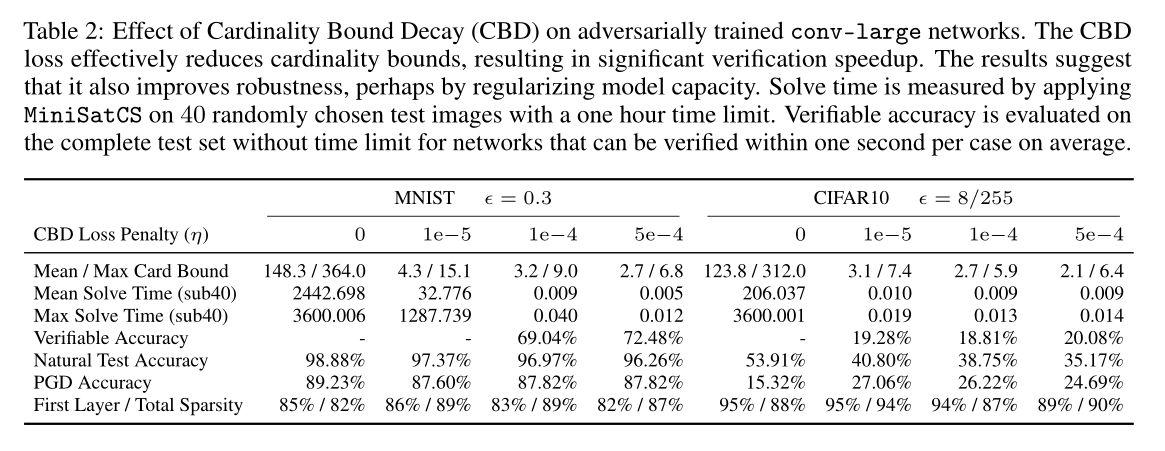
\includegraphics[width=0.9\linewidth]{5.png}
	\end{figure}
\end{frame}

\section{Training verifiably robust BNNs}

\begin{frame}
	\frametitle{Training verifiably robust BNNs}
	\begin{itemize}
		\item Prior work:robust training for real-valued networks (e.g., PGD)
		\item Challenge: A BNN directly trained with PGD has high PGD accuracy, low verifiable accuracy $\implies$ PGD attack becomes ineffective.
		\item This work: adaptive gradient cancelling: $htanh'(x) \to tanh'(x) \to 1- tanh^2(ax)$ ,a is tuned by improving PGD attack success rate
	\end{itemize}
\end{frame}

\begin{frame}
	\frametitle{Training verifiably robust BNNs}
	\begin{figure}
		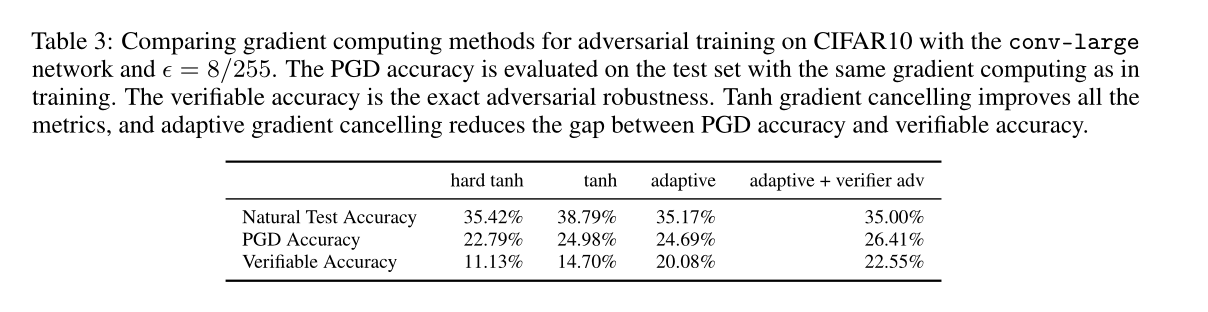
\includegraphics[width=1\linewidth]{6.png}
	\end{figure}
\end{frame}

\section{Other Experiments}
\begin{frame}
	\frametitle{Experiment}
	\begin{figure}
		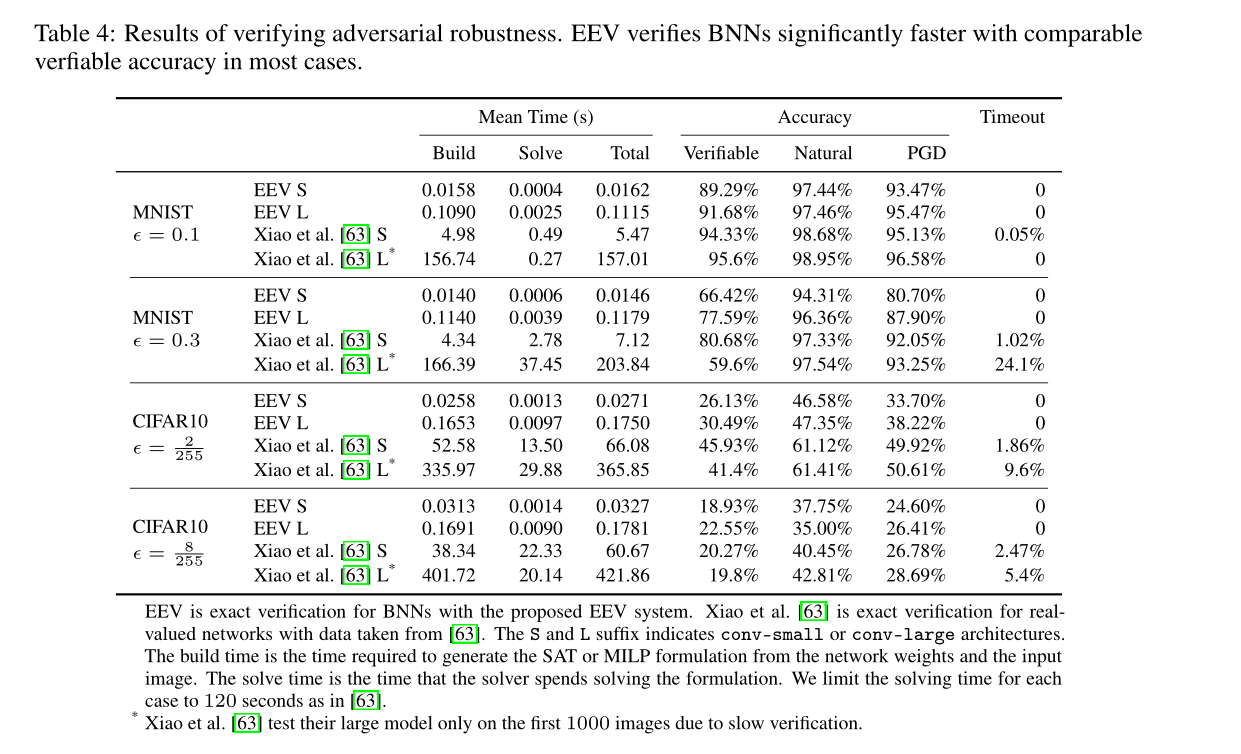
\includegraphics[width=0.75\linewidth]{7.png}
	\end{figure}
\end{frame}

\begin{frame}
	\frametitle{Experiment}
	\begin{figure}
		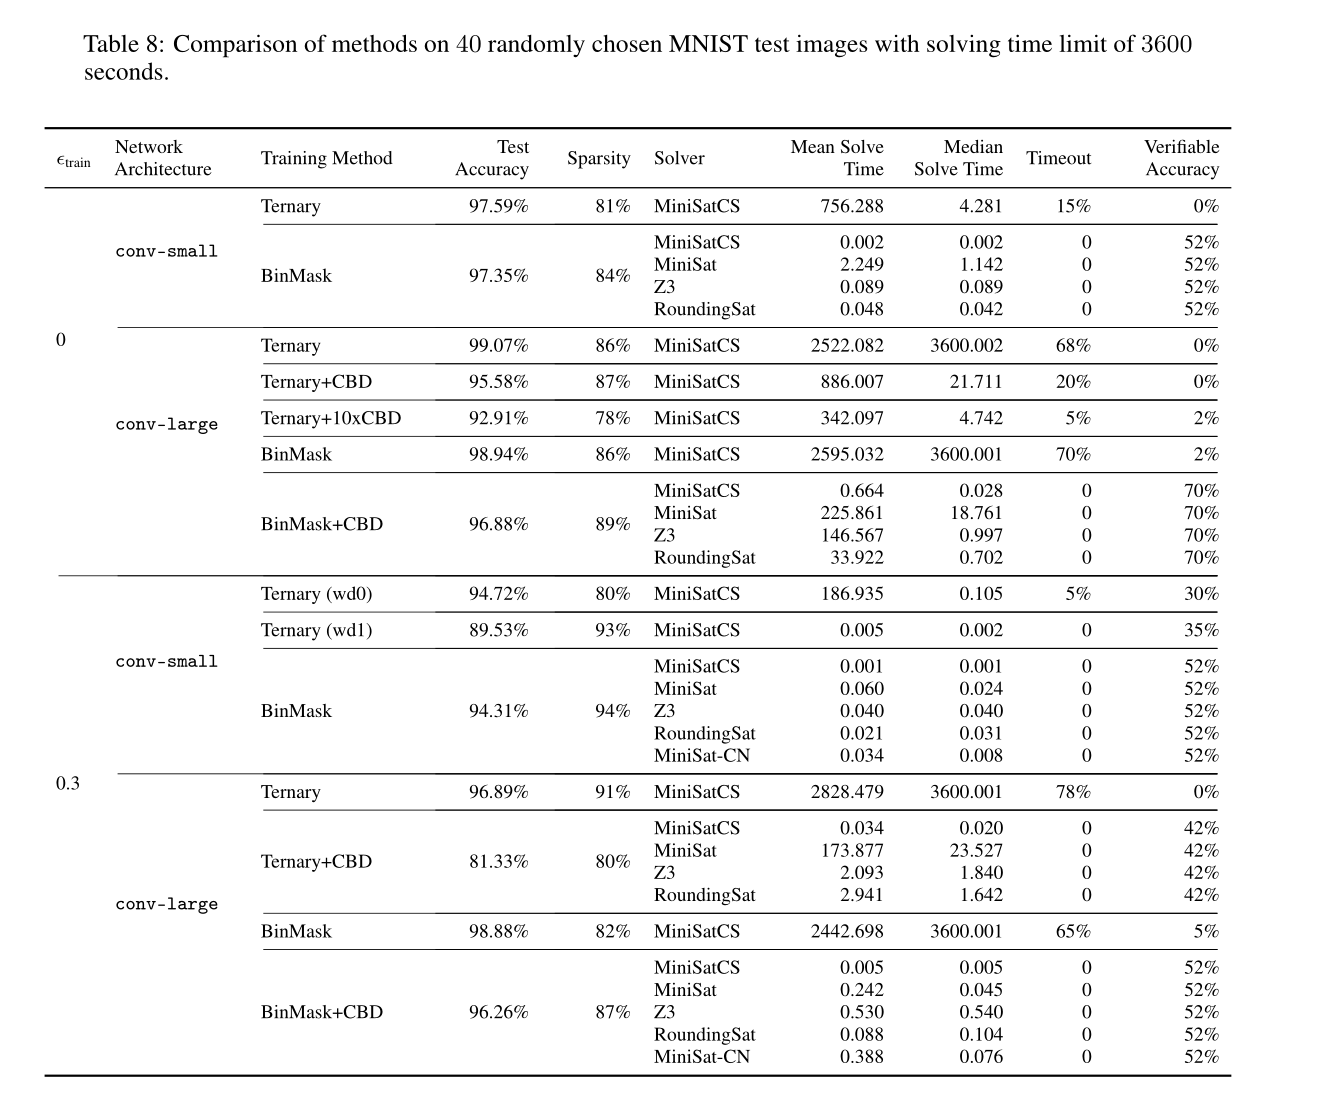
\includegraphics[width=0.75\linewidth]{8.png}
	\end{figure}
\end{frame}

\begin{frame}
	\frametitle{Experiment}
	\begin{figure}
		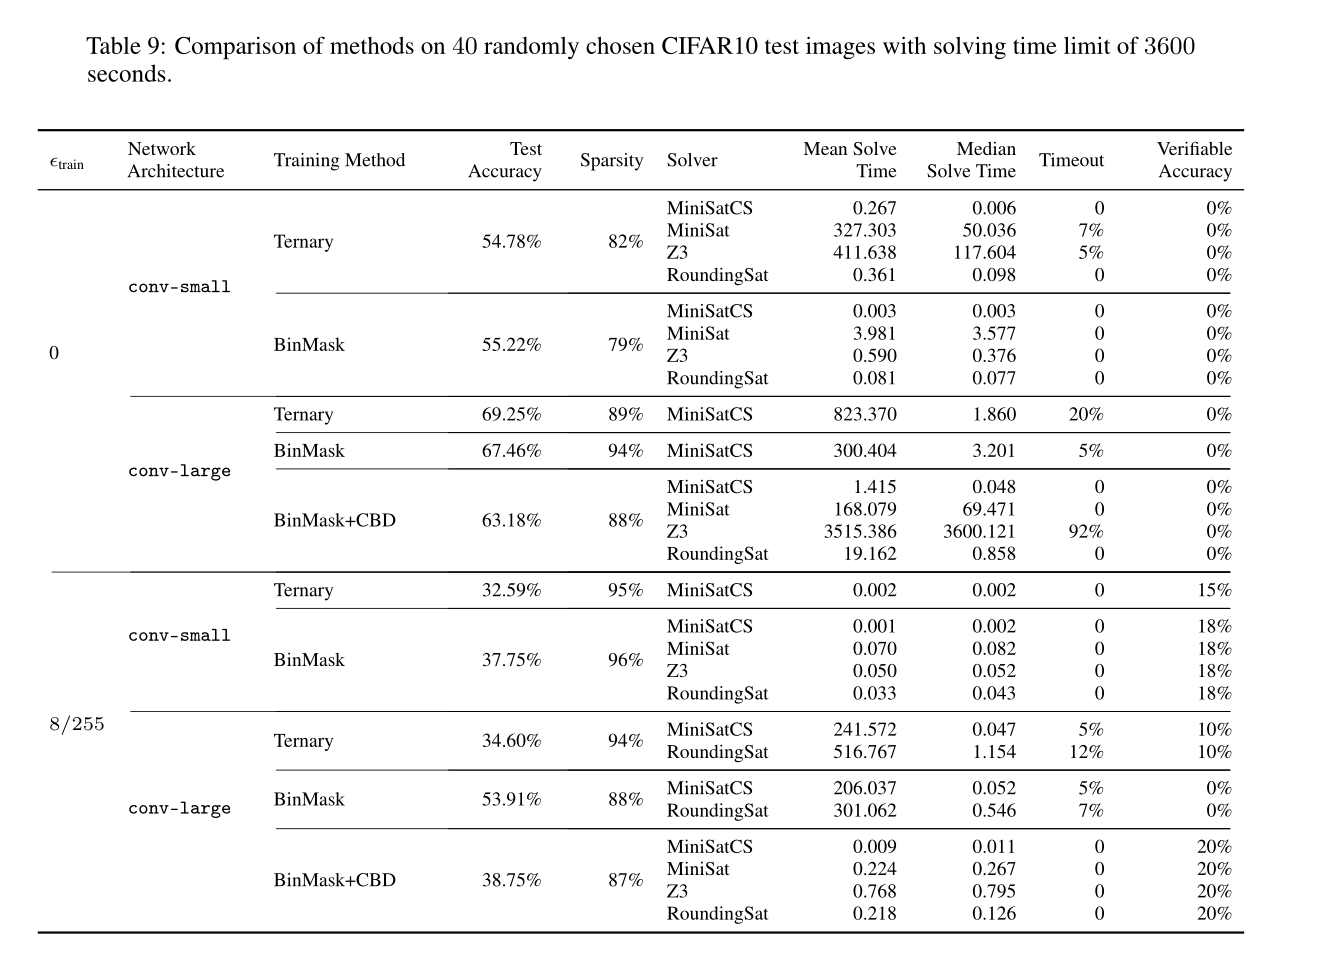
\includegraphics[width=0.75\linewidth]{9.png}
	\end{figure}
\end{frame}
%------------------------------------------------


%------------------------------------------------

%------------------------------------------------


%------------------------------------------------
\begin{frame}
\hfill
\center{\Huge{\calligra{\Huge{Thank you}}}}
\linespread{3}\selectfont
\end{frame}
%----------------------------------------------------------------------------------------
\end{document}